%\section{Prostate Cancer}\label{section:intro:prostatecancer}

%\subsection{Anatomy}\label{subsection:intro:prostatecancer:anatomy}
\section{Prostate anatomy}\label{section:intro:anatomy}

\begin{figure}
\centering
\includegraphics[height=0.25\textheight]{1_introduction/figures/anatomy/prostate2D.eps}
\caption[Sagittal anatomy of prostate.]{Sagittal anatomy scheme of the male reproductive system.}
\label{fig:prostatelocation}
\end{figure}

\begin{figure}
	\centering
	\hspace*{\fill}
	\subfigure[Transverse anatomy of the prostate.]{
			\centering
			\includegraphics[height=0.15\textheight]{1_introduction/figures/anatomy/prostateTransverse.eps}
			\label{fig:anatomyProstateTransverse}}
			\hfill
	\subfigure[Sagittal anatomy of the prostate.]{
			\centering
			\includegraphics[height=0.23\textheight]{1_introduction/figures/anatomy/prostateSagital.eps}
			\label{fig:anatomyProstateSagittal}}\hspace*{\fill}
	\caption[Prostate anatomy.]{Prostate anatomy with division in different zones. \textit{AFT:} anterior fibromuscular tissue, \textit{CZ:} central zone, \textit{ED:} ejaculatory duct, \textit{NVB:} neurovascular bundle, \textit{PUT:}  tissue, \textit{PZ:} peripheral zone, \textit{U:} urethra, \textit{TZ:} transitional zone, \textit{B:} base, \textit{M:} median, \textit{A:} apex (copyright by~\cite{Choi2007}).}
	\label{fig:anatomyProstateZone}
\end{figure}

The prostate is an exocrine gland of the male reproductive system having an inverted pyramidal shape, which is located below the bladder and in front of the rectum as shown in \acs{fig}~\ref{fig:prostatelocation}.
It measures approximately three centimetres in height by two and half centimetres in depth and its weight is estimated to be between seven and sixteen grams for an adult~\cite{Leissner1979}.
The prostate size increases at two distinct stages during physical development: initially at puberty to reach its normal size, then again after sixty years of age leading to \ac{bph}~\cite{Parfait2010}.

A zonal classification of the prostate, depicted in \acs{fig}~\ref{fig:anatomyProstateZone}, was suggested by McNeal\citeauthor{McNeal1981}~\cite{McNeal1981}.
Subsequently, this categorization was widely accepted in the literature~\cite{Hricak1987,Villers1991,Coakley2000,Parfait2010} and is used in all medical examinations (e.g., biopsy, \ac{mri} screening.
The classification is based on dividing the gland into three distinct regions: (i) \ac{cz} accounting for 20-25\% of the whole prostate gland, (ii) \ac{tz} standing for 5\% and (iii) \ac{pz} representing the 70\%.
In \ac{mri} images, tissues of \ac{cz} and \ac{tz} are difficult to distinguish and are usually merged into a common region, denominated \ac{cg}.
As part of this classification, the prostate can be divided in three longitudinal portions depicted in \acs{fig}~\ref{fig:anatomyProstateSagittal}: (i) base, (ii) median gland and (iii) apex.

%% \begin{figure}
%% 	\centering
%% 	\includegraphics[width=0.65\textwidth]{anatomy/prostate2D.eps}
%% 	\caption{Sagittal anatomy scheme of the male reproductive system \cite{Geckomedia2011}.}
%% 	\label{fig:intro:prostatecancer:anatomy:anatomyProstate2D}
%% \end{figure}


%% \begin{figure}
%% 	\centering
%% 	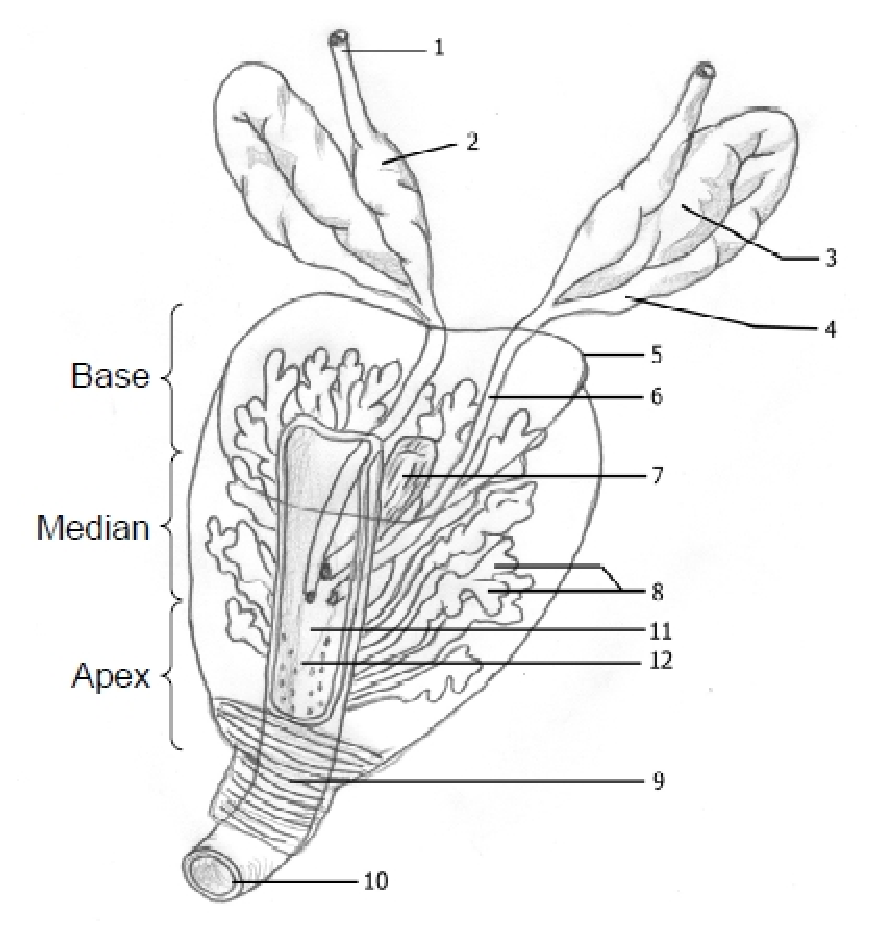
\includegraphics[width=0.50\textwidth]{anatomy/prostate2D2.eps}
%% 	\caption{Representation of the prostate. 1: Vas deferens, 2: Ampulla, 3: Seminal vesicle, 4: Excretory duct of seminal vesicle, 5: Prostate contour, 6: Ejaculatory duct, 7: Prostatic urticle, 8: Glandular tissue, 9: Urethral sphincter, 10: Urethra, 11: Seminal colliculus, 12: Urethral crest \cite{Wikipedia2011}.}
%% 	\label{fig:intro:prostatecancer:anatomy:anatomyProstate2D2}
%% \end{figure}


%% \begin{figure}
%% 	\centering
%% 	\subfigure[Transverse anatomy of the prostate.]{
%% 			\centering
%% 			\includegraphics[width=0.4\textwidth]{anatomy/prostateTransverse.eps}
%% 			\label{fig:anatomyProstateTransverse}}
%% 	~~~
%% 	\subfigure[Sagital anatomy of the prostate.]{
%% 			\centering
%% 			\includegraphics[width=0.4\textwidth]{anatomy/prostateSagital.eps}
%% 			\label{fig:anatomyProstateSagital}}
%% 	\caption{Presentation of the different zones of the prostate. \textit{AFT:} anterior fibromuscular tissue, \textit{CZ:} central zone, \textit{ED:} ejaculatory duct, \textit{NVB:} neurovascular bundle, \textit{PUT:} periurethral tissue, \textit{PZ:} peripherical zone, \textit{U:} urethra, \textit{TZ:} transitional zone \cite{Choi2007}.}
%% 	\label{fig:intro:prostatecancer:anatomy:anatomyProstateZone}
%% \end{figure}

\section{Prostate carcinoma}
Prostate cancer (\acs{cap}) has been reported on a worldwide scale to be the second most frequently diagnosed cancer of men accounting for $13.6 \%$ \cite{Ferlay2010}.
Statistically, in 2008, the number of new diagnosed cases was estimated to be $899,000$ with no less than $258,100$ deaths \cite{Ferlay2010}.
In United States, aside from skin cancer, \ac{cap} was declared to be the most commonly diagnosed cancer among men, implying that approximately one in six men will be diagnosed with \ac{cap} during their lifetime and one in thirty-six will die from this disease causing \ac{cap} to be the second most common cause of cancer death among men \cite{Siegel2013}, \cite{Society2013}.

Despite active research to determine the causes of prostate cancer, a fuzzy list of risk factors has arisen \cite{Society2010}.
The etiology was linked to the following factors \cite{Society2010}: (i) family history \cite{Giovannucci2007,Steinberg1990}, (ii) genetic factors \cite{Freedman2006,Amundadottir2006,Agalliu2009}, (iii) race-ethnicity \cite{Giovannucci2007,Hoffman2001}, (iv) diet \cite{Giovannucci2007,Ma2009,Alexander2010}, and (v) obesity \cite{Giovannucci2007,Rodriguez2007}.
This list of risk factors alone cannot be used to diagnose \ac{cap} and in this way, screening enables early detection and treatment.

\ac{cap} growth is characterized by two main types of evolution \cite{Strum2005}: slow-growing tumours, accounting for up to 85 \% of all \acp{cap} \cite{Lu-Yao2009}, progress slowly and usually stay confined to the prostate gland.
For such cases, treatment can be substituted with active surveillance.
In contrast, the second variant of \acp{cap} develops rapidly and metastasises from prostate gland to others organs, primarily the bones \cite{Oster2013}.
Bone metastases, being an incurable disease, significantly affects the morbidity and mortality rate \cite{Ye2007}.
Hence, the results of the surveillance have to be trustworthy in order to distinguish aggressive from slow-growing \ac{cap}.

\ac{cap} is more likely to come into being in specific regions of the prostate.
In that respect, around 70-80 \% of \acp{cap} originate in \ac{pz} whereas 10-20 \% in \ac{tz} \cite{Carrol1987,McNeal1988,Stamey1998}.
Only about 5 \% of \acp{cap} occur in \ac{cz} \cite{McNeal1988,Cohen2008}.
However, those cancers appear to be more aggressive and more likely to invade other organs due to their location \cite{Cohen2008}.




%%%%%%%%%%%%%%%%%%%%%%%%%% From previous draft %%%%%%%%%%%%%%%%%%%%%%%%%%%%%%%%%%%%%%%%%%%%%%%%

%% \subsection{Statistics}\label{subsection:intro:prostatecancer:statistics}

%% \subsubsection{Overview}\label{subsubsection:intro:prostatecancer:statistics:overview}

%% The World Health Organization (WHO) published in 2008 that PCa was the second most frequently diagnosed cancer of men and the fifth most common cancer overall \cite{Ferlay2010}. No less than 899,000 new cases where detected worldwide in 2008 \cite{Ferlay2010}. As presented on Fig. ~\ref{fig:intro:prostatecancer:statistics:overview:repartitionCancer}, PCa accounts for approximately 7.1\% (Fig. ~\ref{fig:intro:prostatecancer:statistics:overview:repartitionCancerIncidence}) of all cancers diagnosed in 2008 and 3.4\% (Fig. ~\ref{fig:intro:prostatecancer:statistics:overview:repartitionCancerDeaths}) of all cancers deaths in 2008 \cite{Ferlay2010}.

%% \begin{figure}
%% 	\centering
%% 	\subfigure[Estimated number cancers cases for both sexes and all ages.]{
%% 			\centering
%% 			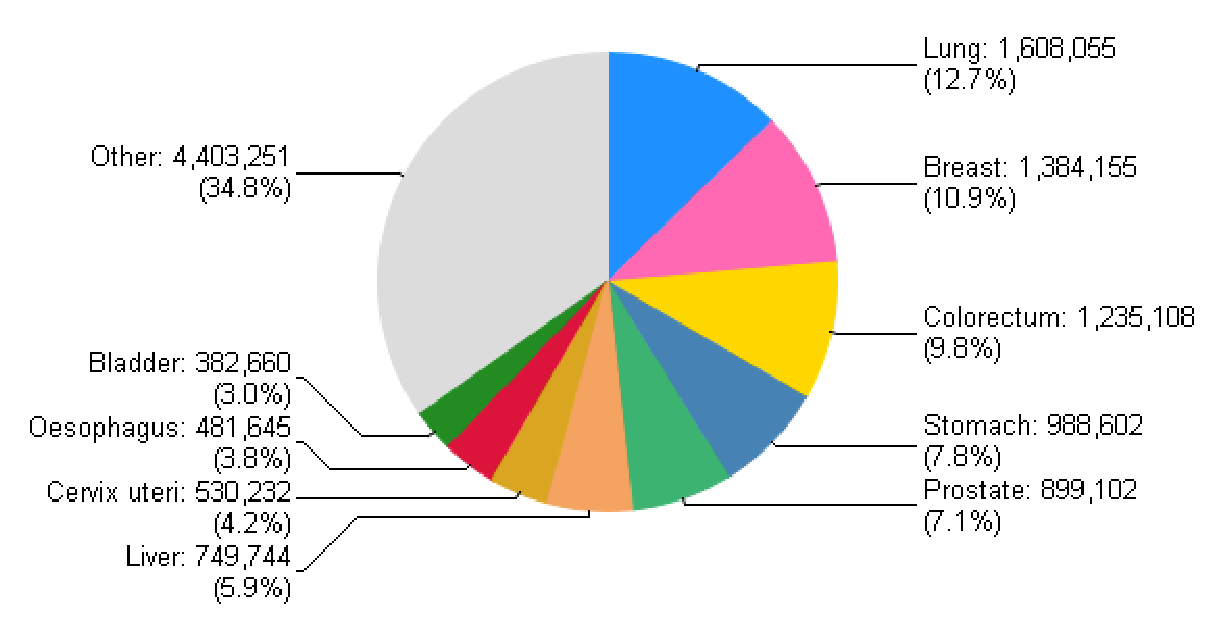
\includegraphics[width=0.65\textwidth]{statistics/repartitionCancerIncidence.eps}
%% 			\label{fig:intro:prostatecancer:statistics:overview:repartitionCancerIncidence}}
%% 	~
%% 	\subfigure[Estimated number cancers deaths for both sexes and all ages.]{
%% 			\centering
%% 			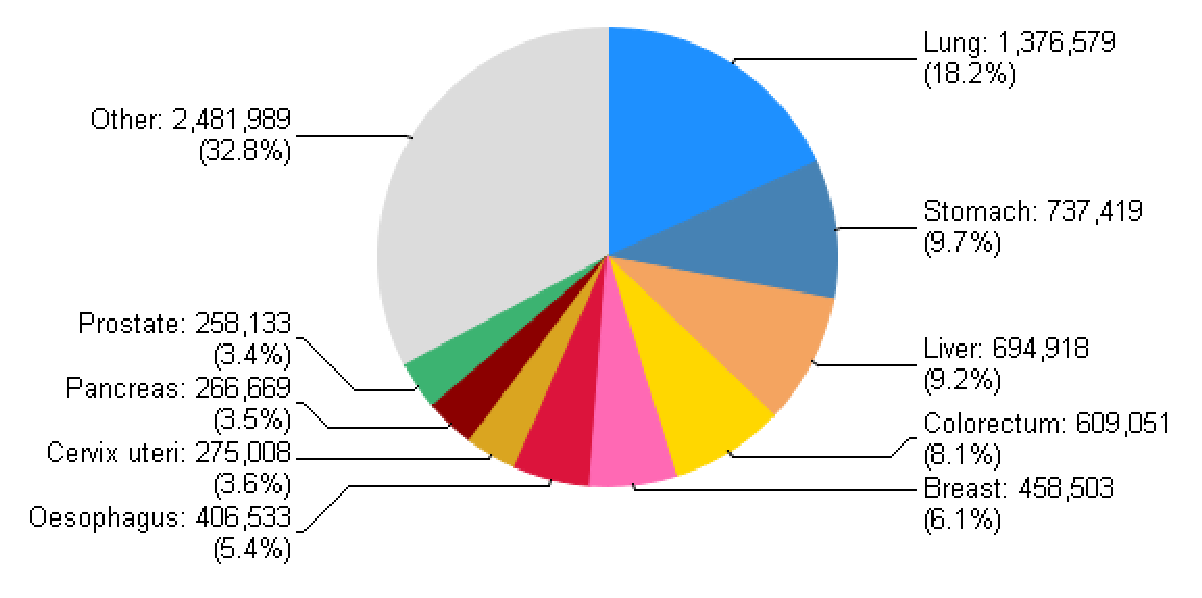
\includegraphics[width=0.65\textwidth]{statistics/repartitionCancerDeaths.eps}
%% 			\label{fig:intro:prostatecancer:statistics:overview:repartitionCancerDeaths}}
%% 	\caption{Cancer estimations in 2008 by the World Health Organization (WHO) \cite{Ferlay2010}.}
%% 	\label{fig:intro:prostatecancer:statistics:overview:repartitionCancer}
%% \end{figure}

%% \subsubsection{Risk Factors}\label{subsubsection:intro:prostatecancer:statistics:riskfactors}

%% The risk factors can be categorized in three different classes: 

%% \begin{itemize}
%% 	\item Age: age is the most important risk factor for PCa. The diagnosis of PCa for men over 50 years old. PCa rate increases upto about 70 and declines thereafter \cite{AmericanCancerSociety2010}.
%% 	\item Genetic factors: it has been shown that the probability to have a cancer is higher when a member of the family has been already diagnosed \cite{AmericanCancerSociety2010}.
%% 	\item Race: in the United States, the Africo Americans have a higher probability of developing a PCa than European American and Hispanic men \cite{AmericanCancerSociety2010}.
%% \end{itemize}

%% \subsection{Diagnosis and Medical Exams}\label{subsubsection:intro:prostatecancer:diagnosis}

%% The presence of PCa may be suggested in several ways: digital rectal examination, Prostate Specific Antigen (PSA\g) test, biopsy using transrectal ultrasound (TRUS\g) and magnetic resonance imaging (MRI\g-MRSI\g).

%% \subsubsection{Digital Rectal Examination}\label{subsubsection:intro:prostatecancer:diagnosis:rectalexamination}
%% Both benign prostatic hyperplasia and cancer may lead to an increasing size of the prostate. A rectal examination may allow detection of harder nodules within the softer prostatic tissue. The advantages are that this method is very fast and does not need any special equipment.
%% \subsubsection{PSA test}\label{subsubsection:intro:prostatecancer:diagnosis:psa}
%% The PSA is a protein secreted by the prostate. A higher-than-normal level of PSA can indicate an abnormality of the prostate: a benign prostatic hyperplasia or a cancer. However, other factors can lead to an increasing level of PSA such as prostate infections, irritations, a recent ejaculation or a recent rectal examination, etc.
%% The PSA can be found in the blood in two different forms: free PSA (about 10\%) and linked to another protein (about 90\%).
%% A level of PSA higher than 10 $ng.mL^{-1}$ is considered as pathologic \cite{Parfait2010}. If the PSA level is between 10 $ng.mL^{-1}$ and 4 $ng.mL^{-1}$, the patient is considered as suspicious \cite{Parfait2010}. In that case, the ratio free PSA over total PSA is computed. If the ratio is higher than 15\%, the case is considered as pathologic.
%% \subsubsection{TRUS}\label{subsubsection:intro:prostatecancer:diagnosis:trus}
%% As described in Sect. ~\ref{subsection:intro:prostatecancer:anatomy}, the prostate is localized in front of the rectum. Hence, its position allows one to carry out a biopsy using transrectal ultrasound (TRUS) in order to localise more precisely an eventual cancer (Fig. ~\ref{fig:intro:prostatecancer:diagnosis:trus}).
%% \textbf{\textit{\textsc{Add example of images of TRUS PCa and not}}}
%% \begin{figure}
%% 	\centering
%% 	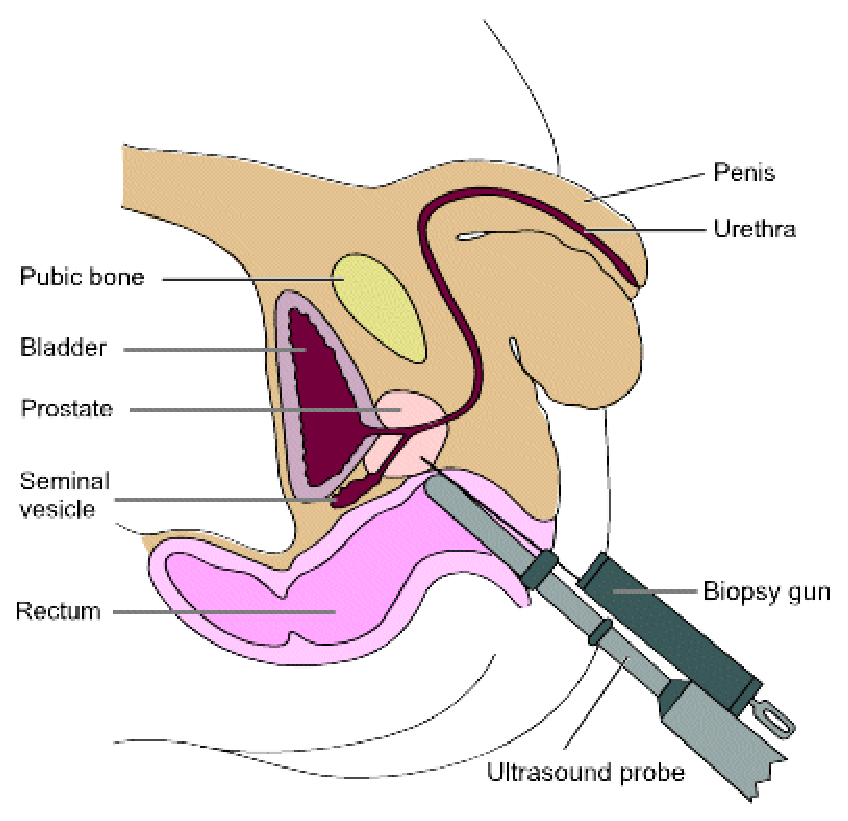
\includegraphics[width=0.45\textwidth]{diagnosis/trus/trus.eps}
%% 	\caption{Biopsy of the prostate using TRUS}
%% 	\label{fig:intro:prostatecancer:diagnosis:trus}
%% \end{figure}
%% \textbf{\textit{\textsc{Add information about protocol: manipulation of the patients, which equipment (see Jhimli thesis)}}}
%% The biopsy is usually prescribed when the PSA level is higher-than-normal or abnormalities were detected during a rectal examination. At least six different samples are taken from the right and left parts of the three different zones: apex, median and base. The samples are analysed in order to determine the presence of a cancer.
%% \textbf{\textit{\textsc{Add more information on the specificities and accuracy of the techniques. Add also what are the advantages (real-time)}}}
